\documentclass[article,12pt]{elsarticle}
\usepackage[spanish]{babel}
\usepackage[utf8]{inputenc}
\usepackage{amssymb}
\usepackage{flushend}
\usepackage{float}
\usepackage{anysize}
\usepackage{amsmath}
\usepackage{amsfonts}
\usepackage{dcolumn}
\usepackage{amsthm}
\usepackage{caption}
\usepackage{float}
\usepackage{subfigure}
\usepackage{graphicx}
\usepackage{lmodern}
\usepackage{booktabs}
\usepackage{color}
\usepackage{longtable}
\usepackage{rotating}
\usepackage{etoolbox}
\usepackage{comment}
\usepackage{pdflscape}
\usepackage{hyperref}
\usepackage{booktabs}


\begin{document}

\begin{frontmatter}
    \title{Laboratorio de Electromagnetismo \\
    Práctica II\\ 
    Líneas equipotenciales}

    \author{Iván Bautista Alvarado$^1$ y Andrés López González$^1$} %Aquí va el nombre de los integrantes que participaron en el informe.
    \address{$^1$ Facultad de Ciencias, Universidad Nacional Autónoma de México, M\'exico CDMX.}

    \begin{abstract}

In this experiment, we investigate the equipotential lines generated by a static electric field in a controlled setup consisting of a negatively charged metal plate and a positively charged coin submerged in water. The primary objective is to visualize and analyze the spatial distribution of these equipotential lines under varying applied voltages (5V, 10V, and 15V). By systematically measuring the electric potential across a two-dimensional grid, we mapped the corresponding equipotential lines and compared the results to theoretical predictions. The experimental data reveal the expected orthogonality between the electric field lines and the equipotential contours, confirming the radial symmetry around the coin and the parallel behavior near the plate. The observed equipotential patterns are consistent with the theoretical framework, demonstrating the influence of charge distribution and geometry on the electric potential landscape. The results not only validate the underlying electrostatic principles but also provide insights into the practical implications of field and potential interactions in complex geometries

    \end{abstract}


    \begin{keyword}
Van de Graaff generator
Energy conversion devices
Electrostatic phenomena
Solar cells efficiency
Thermocouple voltage generation
    \end{keyword}

\end{frontmatter}

    \section*{Resumen}

En este experimento, investigamos las líneas equipotenciales generadas por un campo eléctrico estático en un montaje controlado que consiste en una placa metálica cargada negativamente y una moneda cargada positivamente sumergidas en agua. El objetivo principal es visualizar y analizar la distribución espacial de estas líneas equipotenciales bajo diferentes voltajes aplicados (5V, 10V y 15V). Midiendo sistemáticamente el potencial eléctrico a lo largo de una cuadrícula bidimensional, mapeamos las líneas equipotenciales correspondientes y comparamos los resultados con las predicciones teóricas. Los datos experimentales revelan la ortogonalidad esperada entre las líneas de campo eléctrico y los contornos equipotenciales, confirmando la simetría radial alrededor de la moneda y el comportamiento paralelo cerca de la placa. Los patrones equipotenciales observados son consistentes con el marco teórico, demostrando la influencia de la distribución de carga y la geometría en el paisaje del potencial eléctrico.

\newpage
Los resultados no solo validan los principios electrostáticos subyacentes, sino que también proporcionan ideas sobre las implicaciones prácticas de las interacciones entre campo y potencial en geometrías complejas.\\

\textit{Palabras Clave}: Líneas equipotenciales, Campo electrostático, Distribución de cargas, Mapeo Equipotencial, Geometría del campo.\\ \hline

\section{Introducción}
En el estudio del electromagnetismo se desarrolla uno de los conceptos fundamentales para la física: El concepto de campo.
Para esta práctica, nos situamos en el caso de la electrostática. Para este campo de estudio tenemos al campo eléctrico estático. Para entender este concepto, debemos recordar cómo describimos la fuerza en electrostática. Está dada por la \textit{Fuerza de Coulomb}:
\begin{equation}
    \Vec{F_{1,2}}=k\frac{q_{1}q_{2}}{r_{2,1}^2}\hat{r_{2,1}}
\end{equation}
En donde k es la constante de proporcionalidad quien está estrechamente relacionada a la permitividad del vacío $\epsilon_0$: $k=\frac{1}{4\pi\epsilon_{0}}=8.8543x10^9 N\frac{m^2}{c^2}$. [1]
Y el campo eléctrico que genera una partícula $q_{1}$ está definido como:
\begin{equation}
    \Vec{E}=k\frac{q_{1}}{r_{1,0}^2}\hat{r_{1,0}}
\end{equation}
Podemos ver que tanto el campo como la fuerza son vectores que tienen una forma similar. Pero guardan una importante diferencia. Esta diferencia es que la fuerza solo se puede dar entre dos cargas, y por lo tanto depende de ese par de cargas. En cambio el campo solo depende de una carga y describe el comportamiento de la fuerza eléctrica respecto a una carga de prueba unitaria, además tiene un valor para cada punto del espacio; de esta manera, podemos trazar líneas imaginarias que nos describan el campo eléctrico que genera una partícula (o una cierta densidad de carga) en cada punto del espacio.

Así, podemos relacionar el campo eléctrico con la fuerza mediante la siguiente ecuación:

\begin{equation}
    \Vec{E}=\frac{\Vec{F}}{q_0}
\end{equation}
Esto nos da un indicio de la independencia que tiene el campo eléctrico. Pues es proporcional a la fuerza, pero sin depender de la otra carga.

También es necesario entender otro concepto, del que va a tratar la práctica. El Potencial Electrostático, al que definimos como
\begin{equation}
    \phi(x) = - \int_{P_0}^{x} \Vec{E} \cdot d\Vec{S}
\end{equation}
En donde $\Vec{E}$ es el campo eléctrico generado por una carga, $\Vec{S}$ es la trayectoria que recorre una partícula prueba, que va de un punto ${P_0}$ a un punto de interés ${x}$.

Este nuevo concepto se puede describir como el trabajo por unidad de carga que se tiene que realizar para llevar a una carga de $P_{0}$ a $x$.

El potencial tiene dos características que nos interesan. La primera es que, así como $\Vec{E}$, también es un campo, pero en este caso es un campo escalar, y es dependiente de el punto $P_{0}$ que tomemos como referencia.
Sin embargo, la diferencia de potencial que nos tomamos entre un punto $x_1$ y otro $x_2$ no depende del punto de referencia $P_0$ que tomemos. Esto hace que la diferencia de los potenciales sea una característica especial (A la diferencia de potencial es a lo que llamamos voltaje), y esta es la segunda característica que nos interesa, pues para cualquier campo eléctrico, vamos a tener regiones en las que la diferencia de potencial se mantiene constante, es decir, voltaje constante. Esas regiones se representan como líneas continuas en el espacio, y se les llaman \textit{líneas equipotenciales}.
\\
Podemos relacionar  el potencial con el campo eléctrico y La diferencia de potencial con el campo eléctrico a través de las ecuaciones:
\begin{equation}
    E = \frac{V}{r}
\end{equation}
\begin{equation}
    \Vec{E} = - \nabla \phi
\end{equation}
Sabiendo esto, podemos entender cómo serán las líneas equipotenciales a partir del campo que generan las cargas.\\

Para una lámina cargada, sus líneas de campo se verán así.\\
\begin{figure}[H]
    \centering
    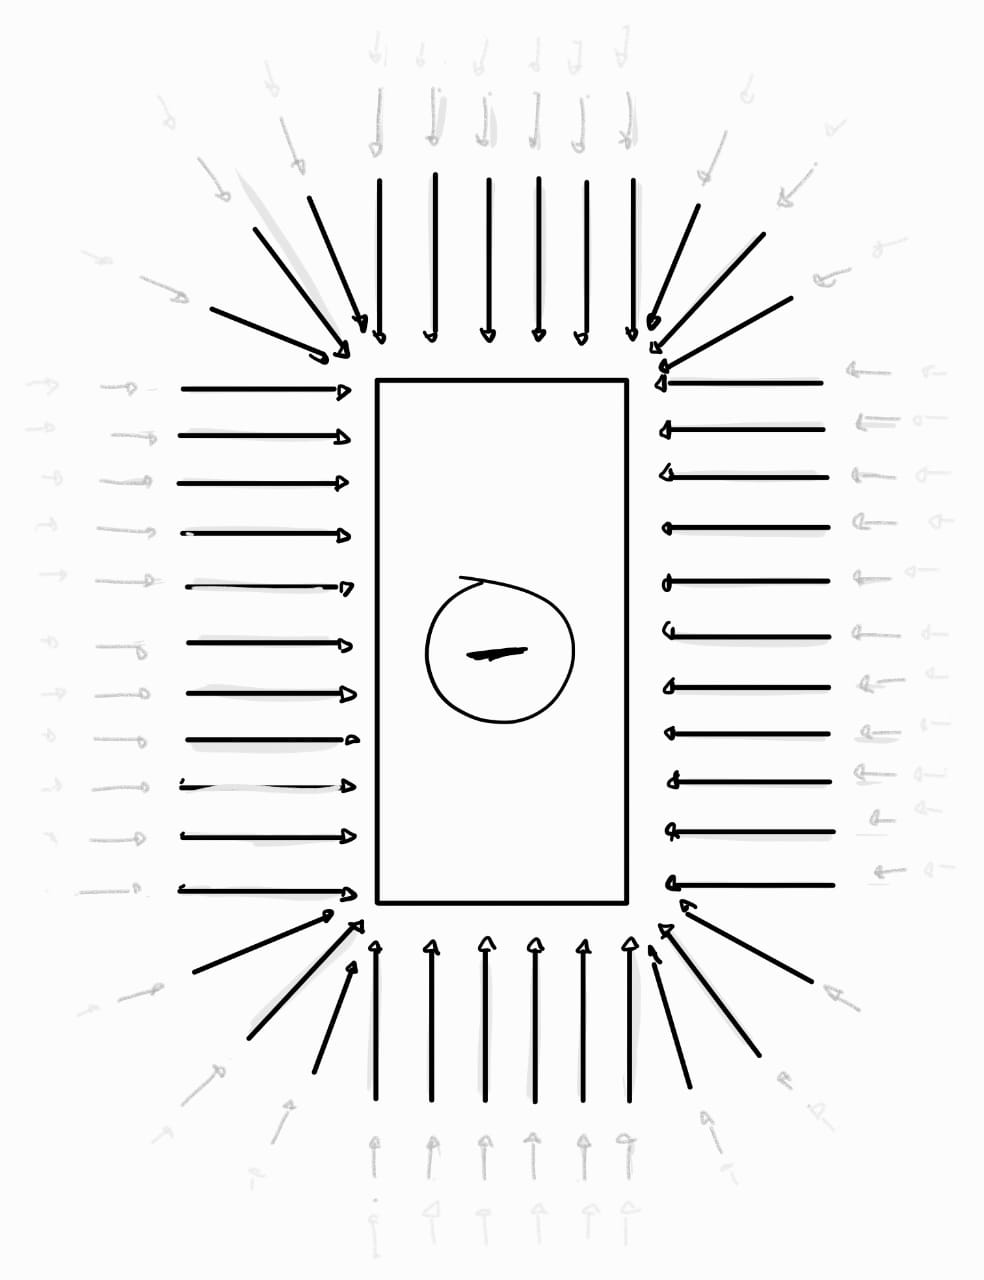
\includegraphics[width=0.35\linewidth]{Lam.png}
    \caption{Líneas de campo de lámina cargada negativamente.}
    \label{fig:enter-label}
\end{figure}
\newpage
Mientras que para una moneda sería de este modo.\\
\begin{figure}[H]
    \centering
    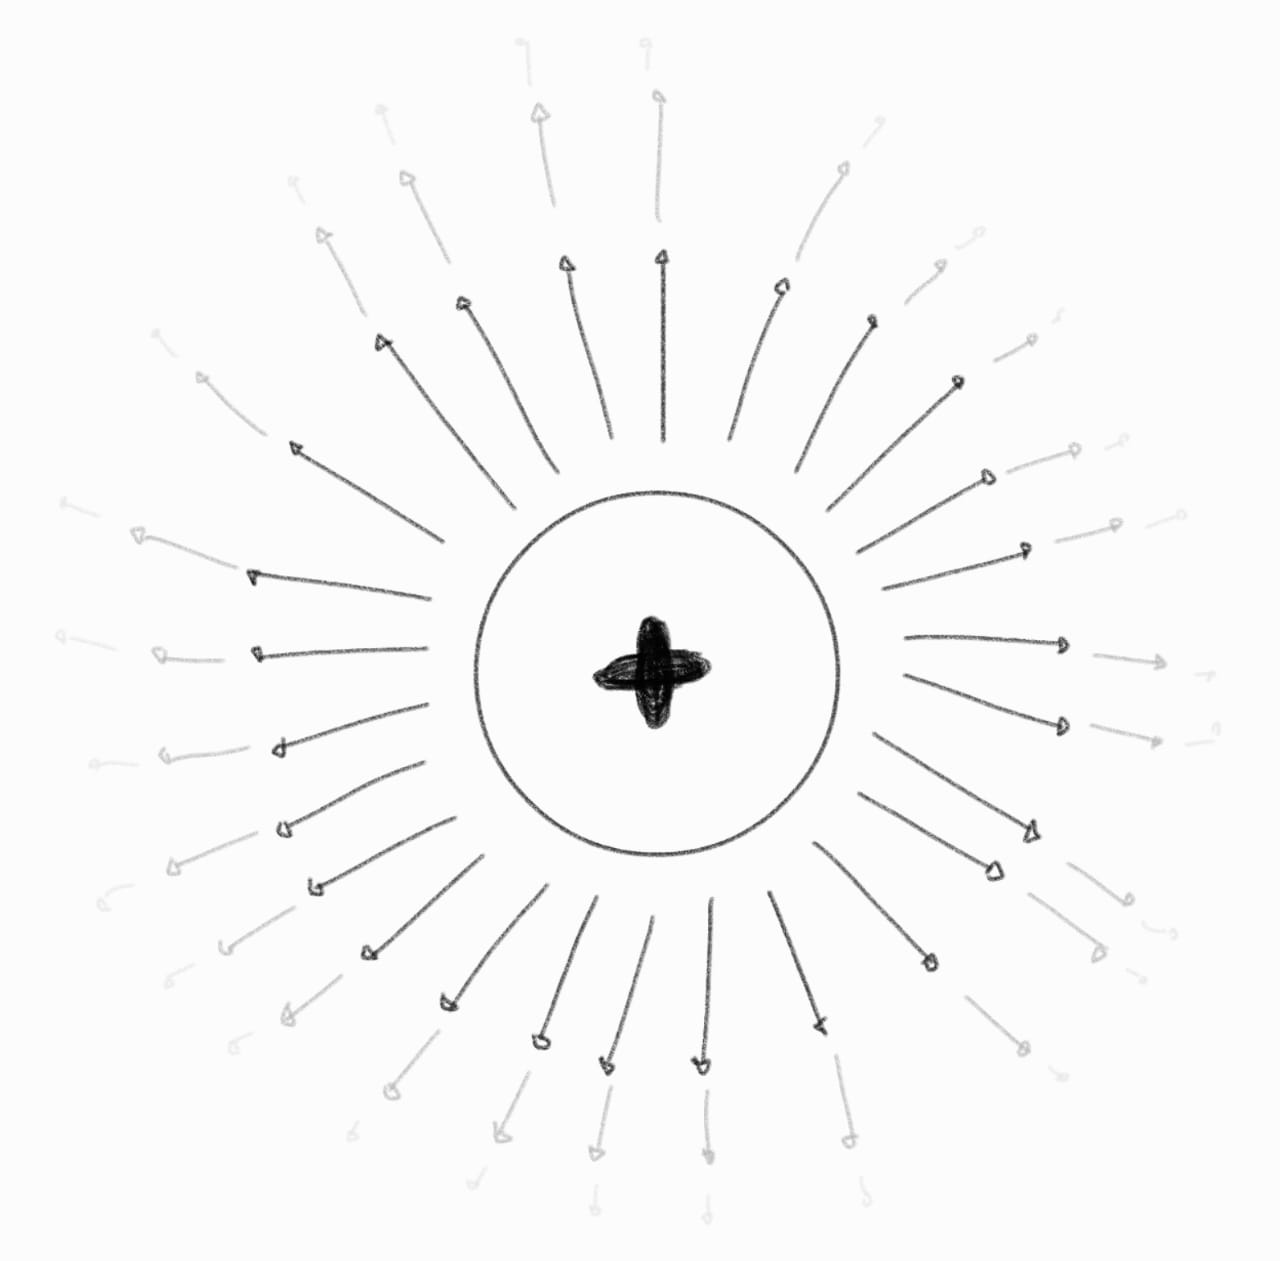
\includegraphics[width=0.4\linewidth]{Moneda.png}
    \caption{Líneas de campo de moneda cargada positivamente.}
    \label{fig:enter-label}
\end{figure}\\
Como el campo eléctrico es ortogonal a las líneas equipotenciales (debido a la ec. 6), podemos predecir cómo serán estas líneas, en consecuencia de Ecuaciones Diferenciales Ordinarias sabemos que para un campo de círculos centrados en el origen (en este caso las líneas equipotenciales) un campo ortogonal a él serán rectas que pasan por el origen de pendiente $m\in \mathbb{R}$ que se verán como vectores radiales; por ello, el comportamiento geométrico que tendrán las líneas equipotenciales será la figura ortogonal a todos nuestros vectores radiales (campo eléctrico) que tengan misma magnitud, quien es una circunferencia. Esto es un poco más impredecible en el caso de la lámina (o placa) pues tenemos una densidad de cargas surgiendo radialmente de cada punto de esta, sin embargo, geométricamente es fácil de observar que las líneas equipotenciales tendrán una apariencia parecida a un rectángulo de bordes suavizados. Para la lámina serán de esta manera.\\
\begin{figure}[H]
    \centering
    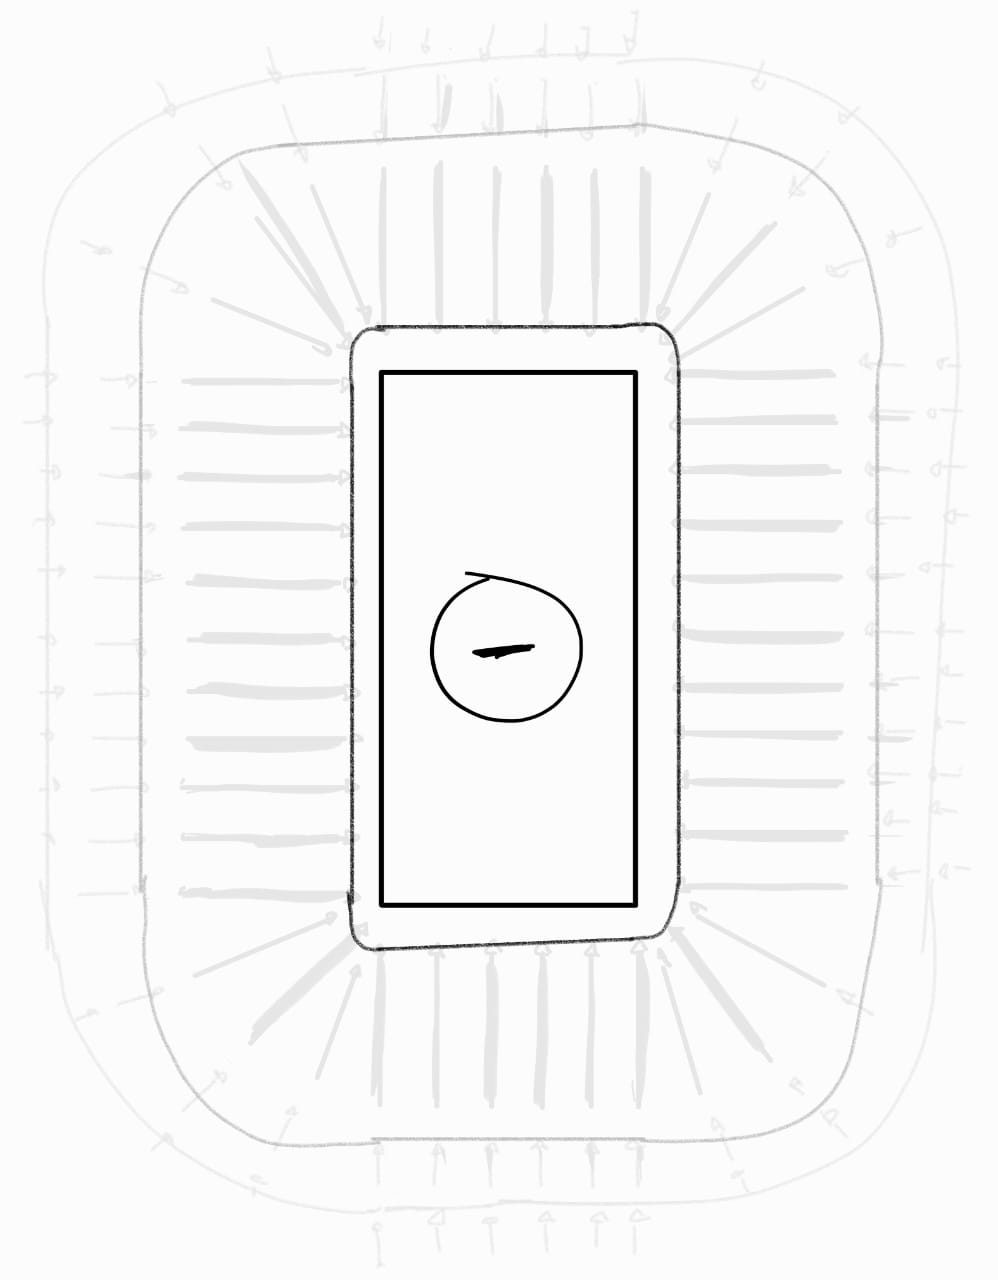
\includegraphics[width=0.35\linewidth]{Lamina EQ.png}
    \caption{Líneas equipotenciales de lámina cargada.}
    \label{fig:enter-label}
\end{figure}\\
Y para la moneda.\\
\begin{figure}[H]
    \centering
    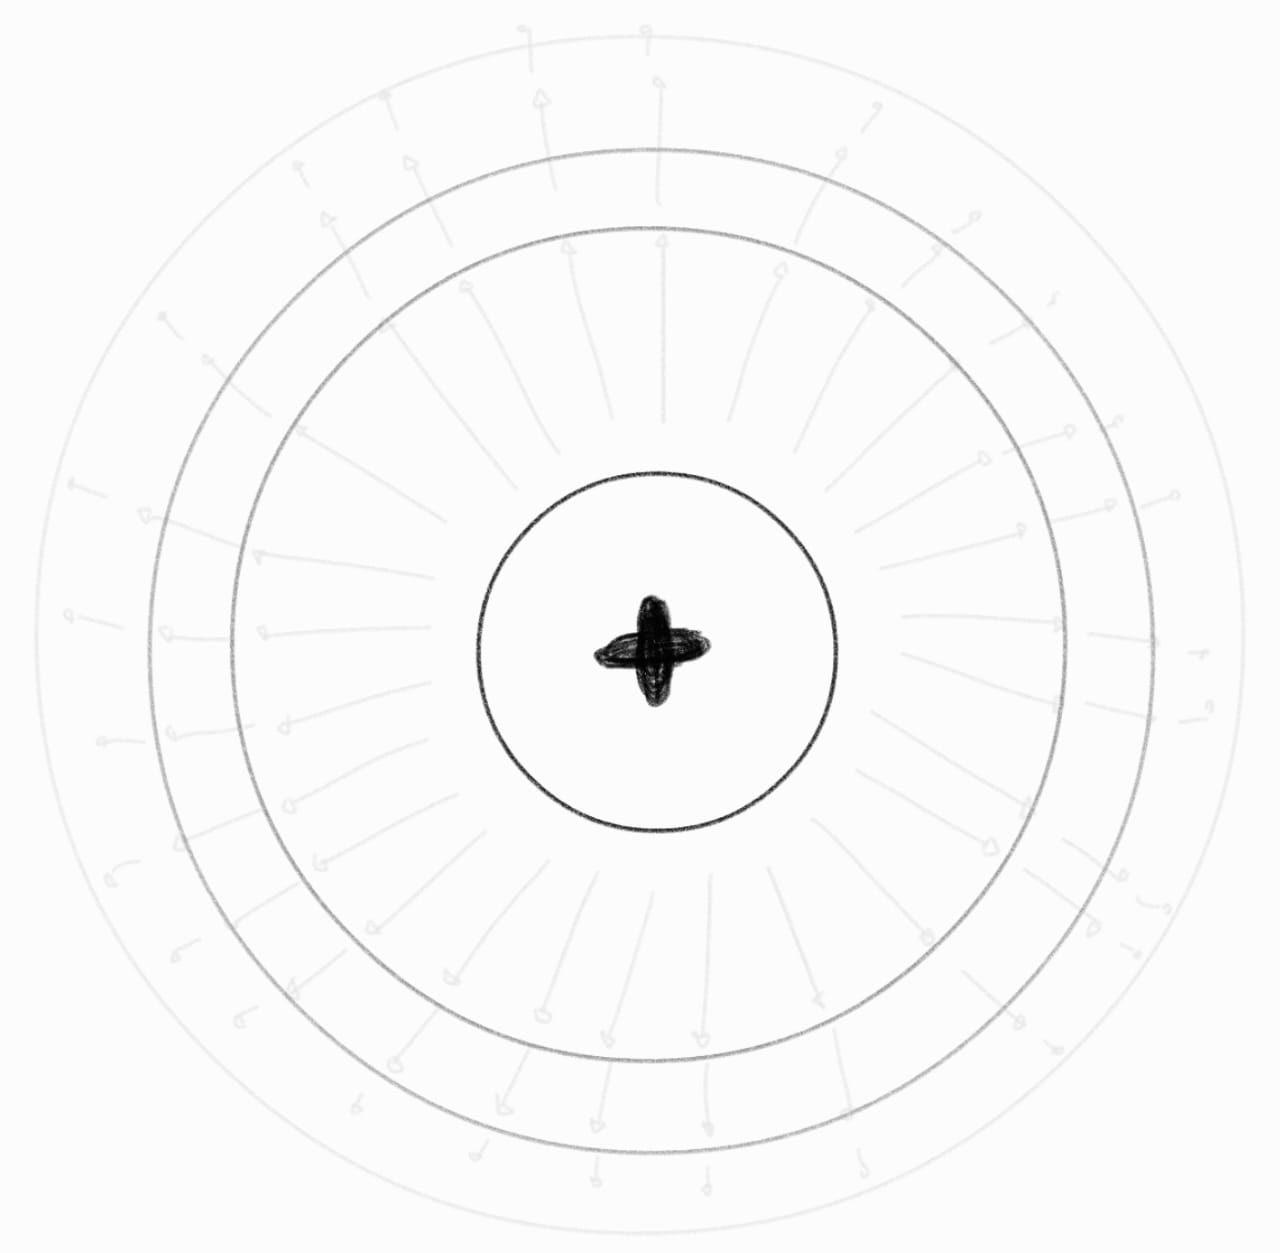
\includegraphics[width=0.3\linewidth]{Moneda EQ.png}
    \caption{Líneas equipotenciales de moneda cargada.}
    \label{fig:enter-label}
\end{figure}\\
Nótese como para nuestro caso placa-moneda al trazar una curva ortogonal a todas las cargas de prueba que generan el mismo campo obtenemos líneas de aproximadamente esta naturaleza.\\
\begin{figure}[h]
    \centering
    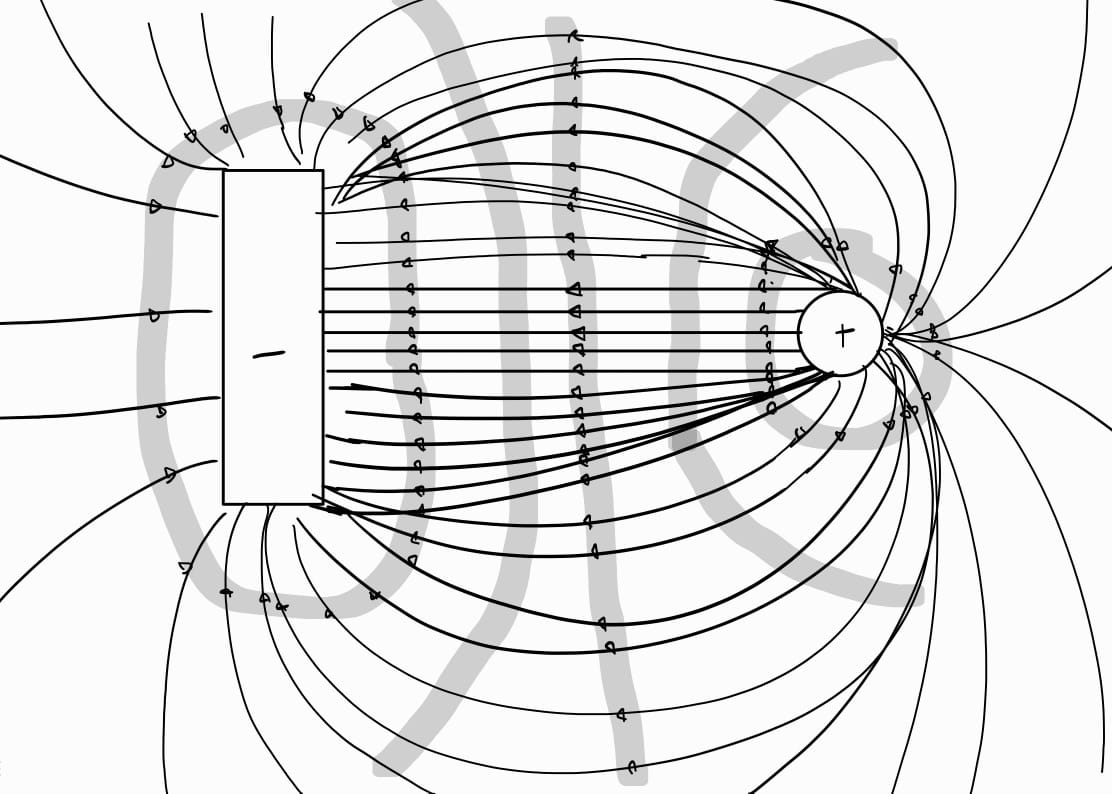
\includegraphics[width=0.5\linewidth]{Diagrama.png}
    \caption{Cómo la teoría indica que son las líneas equipotenciales}
    \label{fig:enter-label}
\end{figure}\\

\subsection{Hipótesis}
A partir del marco teórico que desarrollamos, podemos deducir cómo serán las líneas equipotenciales en el caso del experimento.

Mientras más cerca de la placa esté, las lineas serán parecidas a las que se vieron en el caso de la placa, y mientras nos acercamos a la mitad, esperamos verlas totalmente rectas, pues como una de las superficies tendrá carga negativa y la otra positiva, justo en el medio será donde las lineas de campo tienden a ser paralelas (por ende su línea equipotencial tiende a ser una línea vertical). Y al acercarnos a la moneda se empezará a parecer al diagrama visto para la moneda. \\


\subsection{Objetivos}
Visualizar las líneas equipotenciales que surgen del campo eléctrico estático que genera un arreglo de una placa rectangular de metal cargada negativamente y una moneda cargada positivamente en un medio acuoso.
\section{Desarrollo Experimental / Métodos}
Material utilizado:
\begin{itemize}
    \item 1 Fuente de Voltaje
    \item 1 Multímetro
    \item 1 Refractario de vidrio
    \item 1 Placa de metal ($\approx 2cm \cdot 6cm$ de ancho y alto)
    \item 1 Moneda de $10$
    \item 2 Electrodos
    \item Agua
    \item 2 Pinzas caimanes
    \item Hoja milimétrica (cada cuadrito de $0.\Bar{11}cm$)
\end{itemize}
En el refractario colocamos la moneda y la placa de metal a una distancia de 12cm, y llenamos el refractario de agua hasta que cubriera apenas a los dos objetos, y colocamos la hoja milimétrica debajo del refractario, de tal manera que pudieramos ver las lineas de la hoja y poder guiarnos.

Luego colocamos los electrodos de tal manera que un extremo de ellos tocara a la moneda o a la placa dentro del refractario, y su otro extremo estuviera fuera de este.

A partir de la fuente de voltaje le inducimos la carga a la moneda y a la placa, para esto conectamos sus cables, con las pinzas caimanes a los electrodos. La negativa para la placa y la positiva para la moneda.

Finalmente, ya prendida la fuente de voltaje, usamos el multímetro para detectar el voltaje en los puntos de la superficie acuosa que estaban en medio de los objetos, teniendo la parte negativa de este en la placa y la positiva rastreando la posición de puntos de mismo voltaje como si de un detector de metales se tratase. Primero se fijaron puntos sobre la horizontal entre el centro de la placa y la moneda, siendo el punto de referencia inicial el borde derecho central de la placa, se registraba el voltaje en estos puntos de la horizontal, y luego se rastrearon los puntos en donde el voltaje fuera igual que en esos puntos fijados. Anotando sus posiciones vectoriales y siendo guiados por la hoja milimétrica.   

Esto se realizó para 3 distintos voltajes suministrados por la fuente: 5 volts, 10 volts y 15 volts.

\section{Resultados y discusión}

Para las tres fases de nuestro experimento con 5V, 10V y 15V hemos graficado en un diagrama x vs y con escala en centímetros ($\delta x = \frac{1}{18} cm = \delta y$) las posiciones en donde hemos registrado el mismo valor de voltaje ($\delta V = \frac{1}{2}mV$), de acuerdo a nuestro marco teórico nos dice que estas son nuestras líneas equipotenciales, hemos esbozado el comportamiento de estas curvas para cada caso. \\\\
En nuestra primera fase de 5V registramos 1.60V en nuestra posición (0,2), i.e. a 2 centímetros respecto al borde central de la placa, por lo que la primera curva corresponde a los puntos que obtuvieron este mismo voltaje. Análogamente para (0,4) en donde se registró 2.07V, en (0,6) se registró 2.59V, para (0,8) que es a 4cm de la moneda se registró 3.10V y finalmente para (0,10) quien es a 2cm de la moneda se registró 3.72V. Por curiosidad medimos sobre la moneda en donde se obtuvo 4.97V, lo cual nos confirmó que efectivamente se han tomado con muy buena precisión las mediciones y por ende nuestra descripción de las líneas equipotenciales es fiel al fenómeno.
\begin{figure}[H]
    \centering
    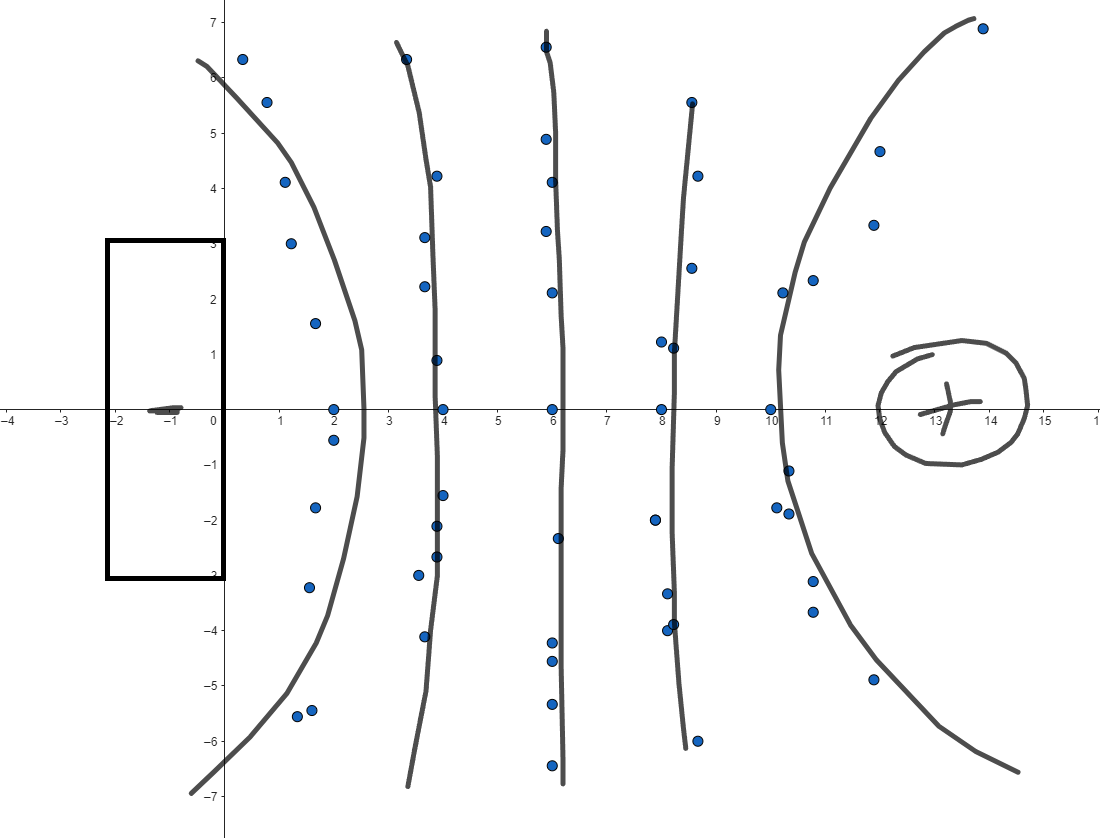
\includegraphics[width=0.75\linewidth]{5V EQ.png}
    \caption{Enter Caption}
    \label{fig:enter-label}
\end{figure}\\

\textit{Nota: Nuestra convención de curvas (distanciadas cada 2 cm respecto al borde central derecho de la placa) y distancias respecto a la moneda/placa de metal, se mantiene para las demás fases, por lo que una vez explicada esta convención, se registró en una tabla sus voltajes para agilizar el análisis.}\\

\newpage
Para la segunda fase véase en la tabla los voltajes correspondientes a cada línea equipotencial y la gráfica de los puntos que satisfacen tener la misma carga.\\
\begin{table}[h]
\begin{tabular}{l|l}
$\#$Curva & Voltaje asociado \\ \hline \hline
Primera Curva & 2.70V \\
Segunda Curva & 3.94V \\
Tercera Curva & 5.38V \\
Cuarta Curva  & 6.43V \\
Quinta Curva  & 7.65V
\end{tabular}
\end{table}\\
\begin{figure}[h]
    \centering
    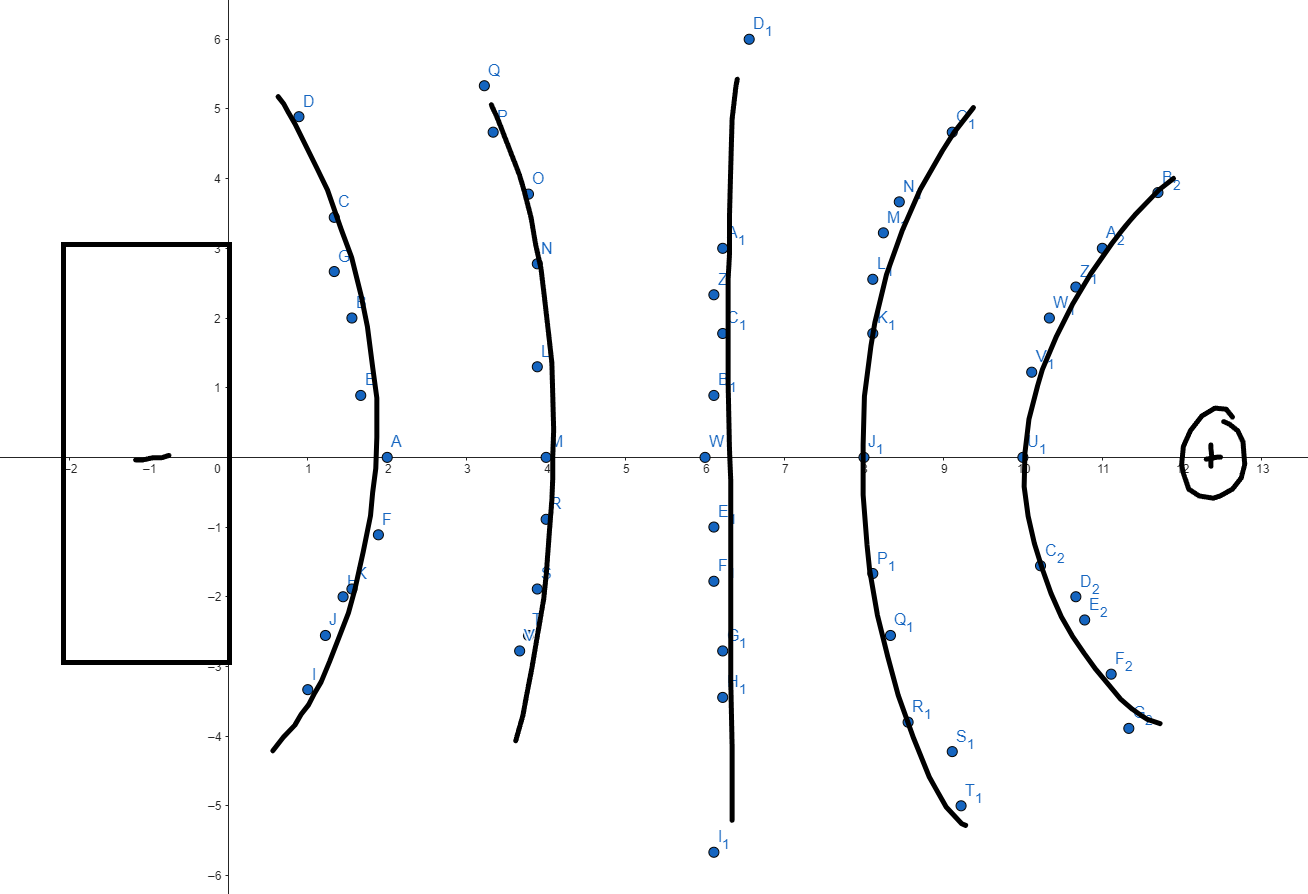
\includegraphics[width=0.85\linewidth]{10V EQ.png}
    \caption{Enter Caption}
    \label{fig:enter-label}
\end{figure}\\

Finalmente para nuestra tercera fase a 15V tenemos la siguiente tabla del voltaje asociado a cada curva equipotencial y su gráfica.\\

\begin{table}[h]
\begin{tabular}{l|l}
$\#$Curva & Voltaje asociado \\ \hline \hline
Primera Curva & 4.00V \\
Segunda Curva & 5.71V \\
Tercera Curva & 7.55V \\
Cuarta Curva  & 9.53V \\
Quinta Curva  & 11.32V
\end{tabular}
\end{table}\\

%%DISCUSION DE RESULTADOS

\begin{figure}[H]
    \centering
    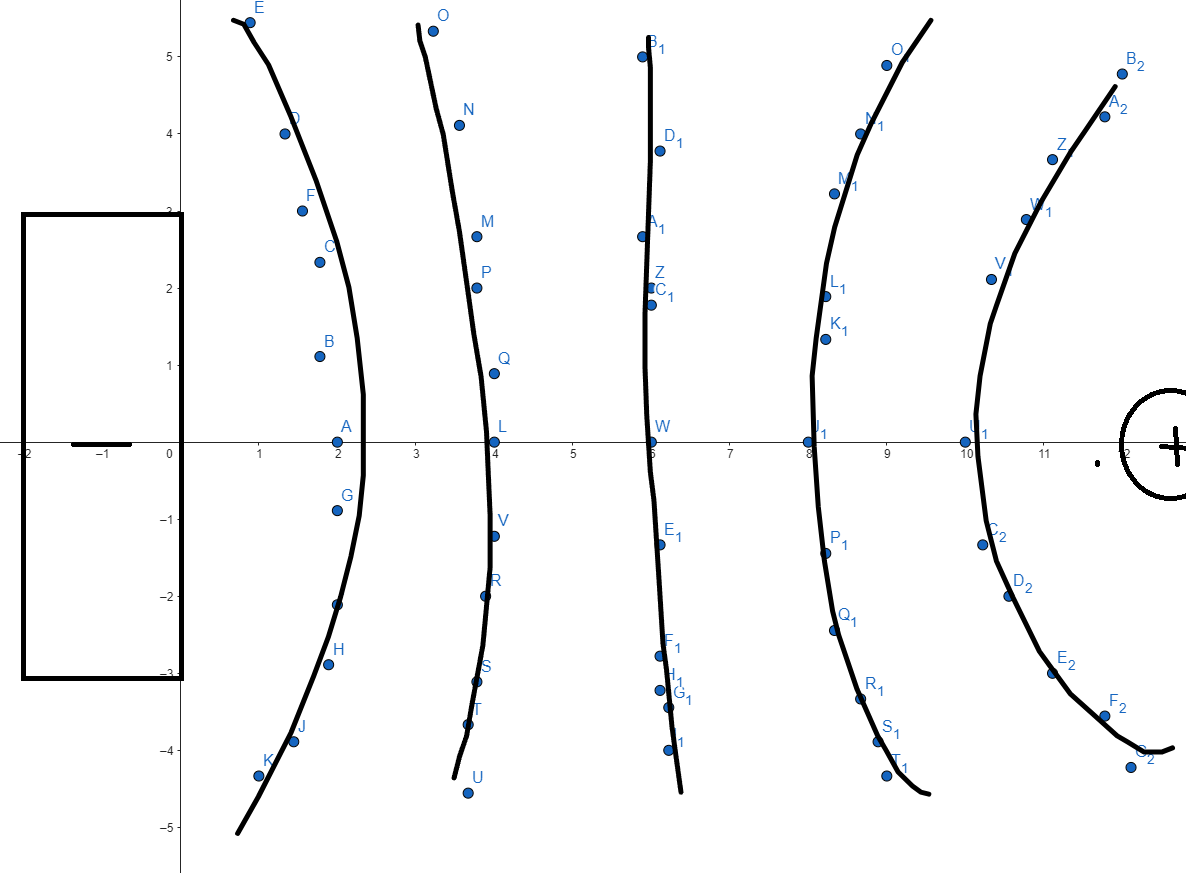
\includegraphics[width=0.75\linewidth]{15V EQ.png}
    \caption{Enter Caption}
    \label{fig:enter-label}
\end{figure}\\

\section{Conclusiones}
Las gráficas resultantes del experimento siguen la descripción que sugeríamos en la hipótesis. Cuando registrábamos cerca del centro de la placa, las lineas se acercaban a ser paralelas, y mientras nos acercábamos al borde de la placa, se empezaban a curvar más. Siendo parecido al diagrama mostrado en la Figura 3 pero sin ser tan exagerado, además de presentar ciertas irregularidades notorias muy potencialmente causadas por la geometría imperfecta de esta placa.\\
De la misma manera, la gráfica al acercanos a la moneda se curva de una manera más intensa, resultando casi idéntico al diagrama de la Figura 4, es importante ver que la moneda no presenta fallos visuales en su geometría por lo que al tener un instrumento de medición tan preciso (1 mV como mínima escala) asociamos las anomalías con la pureza y forma de la placa; bajo la hipótesis de la electrostática (cargas sin movimiento) el desarrollo del marco teórico ayudó a predecir de manera correcta el comportamiento de las lineas equipotenciales.
\newpage
\noindent {\bf Declaración de contribución de los autores}\\ 

Iván Bautista Alvarado$^1$ y Andrés López González$^1$ hemos realizado tanto el apartado escrito como el análisis de manera colectiva siendo una participación del 100\% por parte de ambos y no solo una repartición.\\ 

{\bf Agradecimientos} \\ 

A ese.\\

\begin{figure}[H]
    \centering
    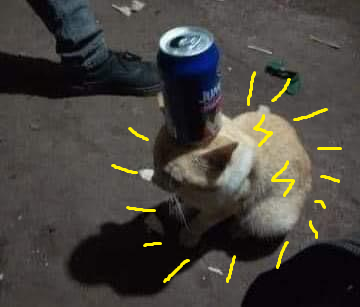
\includegraphics[width=0.5\linewidth]{el.png}
    \caption{Electrogato}
    \label{fig:enter-label}
\end{figure}\\

\begin{thebibliography}{99}

\bibitem{griffiths}
D. J. Griffiths, \textit{Introduction to Electrodynamics}, 3rd ed. Upper Saddle River, NJ, USA: Prentice-Hall, 1999.

\bibitem{jackson}
J. D. Jackson, \textit{Classical Electrodynamics}, 3rd ed. New York, NY, USA: Wiley, 1998.

\bibitem{sadiku}
M. N. O. Sadiku, \textit{Elements of Electromagnetics}, 6th ed. New York, NY, USA: Oxford University Press, 2014.

\bibitem{wangsness}
R. K. Wangsness, \textit{Electromagnetic Fields}, 2nd ed. New York, NY, USA: Wiley, 1986.

\bibitem{zangwill}
A. Zangwill, \textit{Modern Electrodynamics}. Cambridge, UK: Cambridge University Press, 2013.

\bibitem{purcell}
E. M. Purcell and D. J. Morin, \textit{Electricity and Magnetism}, 3rd ed. Cambridge, UK: Cambridge University Press, 2013.

\bibitem{shadowitz}
A. Shadowitz, \textit{The Electromagnetic Field}. Mineola, NY, USA: Dover Publications, 1988.

\end{thebibliography}

\appendix
\section{Creación del gráfico}
\label{app1}

Debido a que se registraron una cantidad abrumadora para el lector de posiciones vectoriales hemos decidido incluir estos gráficos sin líneas trazadas en el apéndice. Adjunto el enlace de geogebra correspondiente a cada uno de mis gráficos para poder visualizar la posición exacta de cada uno de estos puntos, en cada gráfico se han usado 11 mediciones por línea equipotencial para mantener la curva lo más fiel posible a la realidad. \\
Nótese que los decimales son periódicos pues son novenos de centímetros debido al tipo de hoja milimétrica que se ha usado ($0.\Bar{11}cm =\frac{1}{9}cm$ como mínima escala).

\begin{figure}[h]
    \centering
    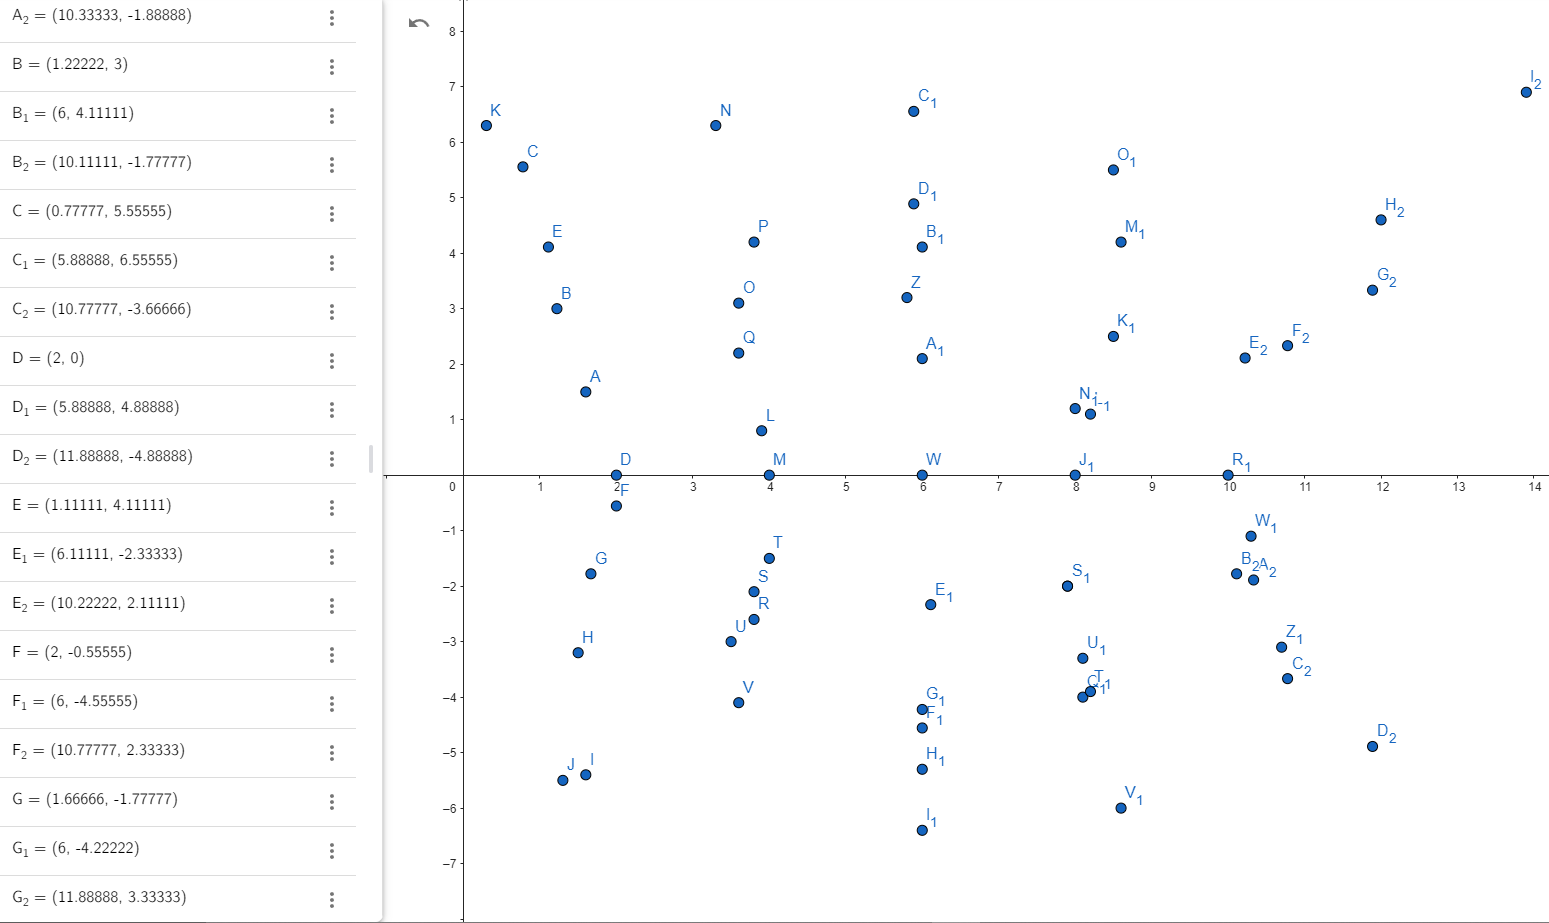
\includegraphics[width=1\linewidth]{5V des.png}
    \caption{Gráfico de 5V \href{https://www.geogebra.org/graphing/a6699hbp}{https://www.geogebra.org/graphing/a6699hbp}}
    \label{fig:enter-label}
\end{figure}\\

\begin{figure}[h]
    \centering
    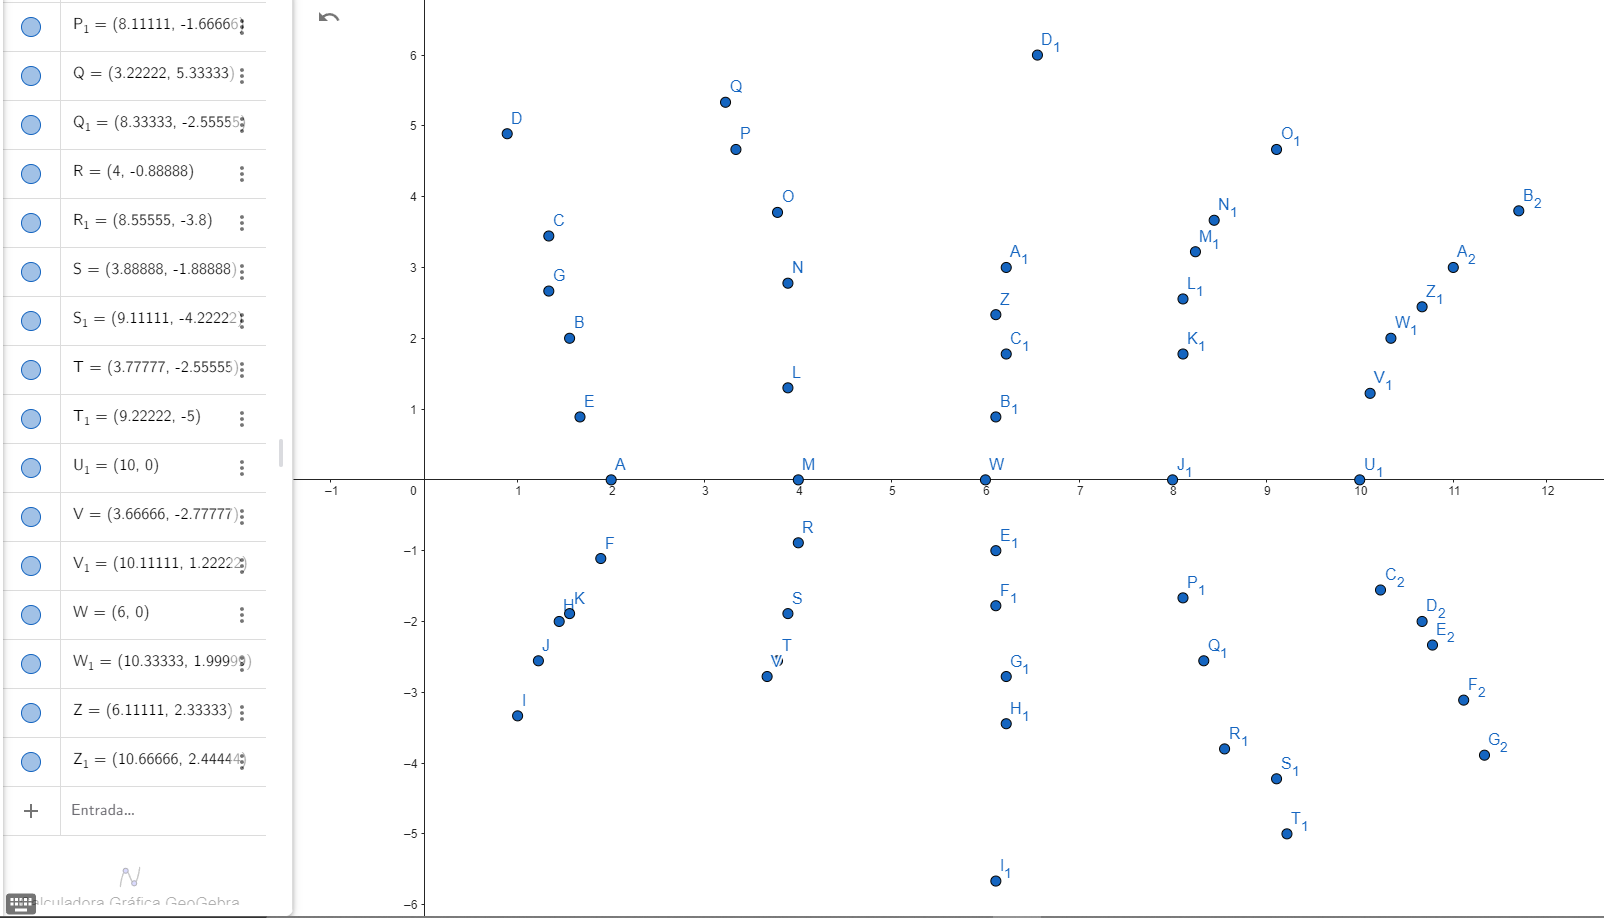
\includegraphics[width=1\linewidth]{10V des.png}
    \caption{Gráfico de 10V \href{https://www.geogebra.org/graphing/f5errmjx}{https://www.geogebra.org/graphing/f5errmjx}}
    \label{fig:enter-label}
\end{figure}

\begin{figure}
    \centering
    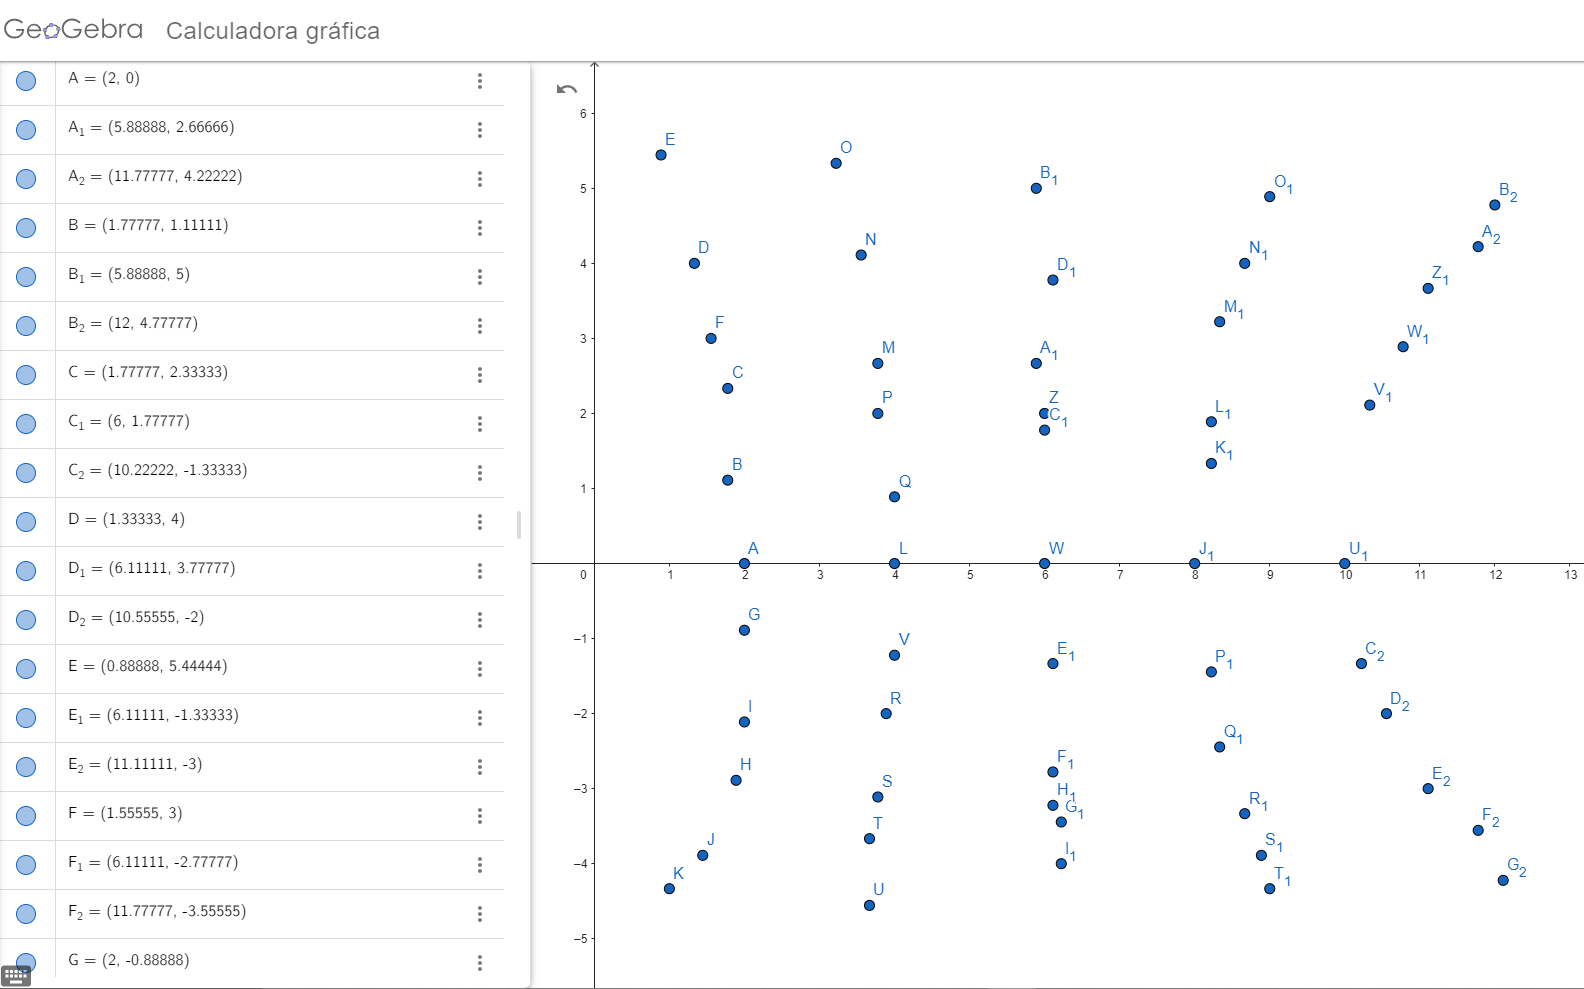
\includegraphics[width=1\linewidth]{15V des.png}
    \caption{Gráfico de 15V \href{https://www.geogebra.org/graphing/tyny8bfm}{https://www.geogebra.org/graphing/tyny8bfm}}
    \label{fig:enter-label}
\end{figure}



\end{document}